
\documentclass[11pt,serif,aspectratio=169]{beamer}

% Set the margins to be something normal.
% \usepackage[margin=1in]{geometry}

% Fun lists!
\usepackage{enumitem}
\usepackage{textcomp}
\setitemize{label=\textrightarrow, itemsep=0pt}

% Math symbols.
\usepackage{amsmath,amssymb,amsfonts,tikz,mathtools,pgfplots,nicefrac}
\pgfplotsset{compat=newest}
\usetikzlibrary{shapes,arrows,positioning,calc}  
\usetikzlibrary{overlay-beamer-styles}

% No indents.
\setlength\parindent{0pt}
\setlength\parskip{1em}

\newcommand{\inverse}[1]{#1^{-1}}


% Nice fonts :)
%\usepackage{tgschola}
\usefonttheme[onlymath]{serif}

\begin{document}
	\begin{frame}[c]\centering \Large \bf
		exam 2 review
	\end{frame}
	
	\begin{frame}[c]\centering \Large \bf
		8.2 --- integration by parts
	\end{frame}
	
	\begin{frame}[c]{the product rule} \Large
		$$ \frac{d}{dx}\left(u(x) \cdot v(x)\right) = u(x) \cdot v'(x) + u'(x) \cdot v(x) $$
	\end{frame}
	
	\begin{frame}[c]{\textit{integrating} the product rule}\centering \Large \bf
		\begin{align*}
			\onslide<1->{\int \frac{d}{dx}\left( u(x) \cdot v(x) \right) & = \int \left(u(x) \cdot v'(x) + u'(x) \cdot v(x) \right) dx	\\}
			\onslide<2->{u(x) \cdot v(x) & = \boxed{\int u(x) \cdot v'(x) dx} + \boxed{\int u'(x) \cdot v(x) dx} \\[2em]}
			\onslide<3->{\boxed{\int u(x)\cdot v'(x) dx} &= u(x) \cdot v(x) - \boxed{\int u'(x) \cdot v(x) dx}}
		\end{align*}
	\end{frame}	
	
	\begin{frame}[c]{2(b), old exam 2} \Large
		$$ \int x^2 \cos x \ dx $$	
	\end{frame}
	
	\begin{frame}[c] \Large
		\onslide<1->{ $$u = x^2, \ dv = \cos(x) dx$$} \onslide<2->{$$\implies du = 2x dx, \ v = \sin(x)$$}
	\end{frame}
	
	\begin{frame}[c]{2(b), old exam 2} \Large
		\begin{align*}
			\onslide<1->{\int udv &= uv - \int v du \\}
			\onslide<2->{\int x^2 \cos(x) dx &= x^2 \sin(x) - \int 2x \sin(x) dx}
		\end{align*}	
	\end{frame}
	
	\begin{frame}[c]{2(b), old exam 2} \Large
		\onslide<1->{ $$u = 2x, \ dv = -\sin(x) dx$$} \onslide<2->{$$\implies du = 2 dx, \ v = \cos(x)$$}
	\end{frame}
	
	\begin{frame}[c]{2(b), old exam 2} \Large
		\begin{align*}
			\onslide<1->{\int udv &= uv - \int v du \\
			\int x^2 \cos(x) dx &= x^2 \sin(x) - \int 2x \sin(x) dx \\}
			\onslide<3->{&= x^2 \sin(x) + 2x\cos(x) - \int 2\cos(x) dx \\}
			\onslide<4->{&= x^2 \sin(x) + 2x\cos(x) - 2 \sin(x) + C}
		\end{align*}	
	\end{frame}
	
	\begin{frame}[c] \centering \Large \bf
		8.3, 8.4 --- trig integrals and substitution
	\end{frame}
	
	\begin{frame} \Large
		\begin{figure}[h!]
			\scalebox{0.7}{
				\begin{tikzpicture}
					\draw (0,0) node[anchor=north]{}
						-- (4, 0) node{}
						-- (4, 3) node{}
						-- cycle;
						
					\node at (2,-1/4) {$a$};
					\node at (4.25, 1.5) {$x$};
					\node at (0, 1.5) {$\sqrt{x^2 + a^2}$};
					\node at (2.5, 1) {$A$};
					\node at (0.75, 0.25) {$\theta$};
					\draw (3.7,0)|-(4,0.3);
					
					% Triangle 2
					\draw (6,0) node[anchor=north]{}
						-- (10, 0) node{}
						-- (10, 3) node{}
						-- cycle;
						
					\node at (8,-3/4) {$\sqrt{a^2-x^2}$};
					\node at (10.25, 1.5) {$x$};
					\node at (7.5, 1.5) {$a$};
					\node at (8.5, 1) {$B$};
					\node at (6.75, 0.25) {$\theta$};
					\draw (9.7,0)|-(10,0.3);
					
					% Triangle 3
					\draw (12,0) node[anchor=north]{}
						-- (16, 0) node{}
						-- (16, 3) node{}
						-- cycle;
						
					\node at (14,-1/4) {$a$};
					\node at (17.25, 1.5) {$\sqrt{x^2-a^2}$};
					\node at (13.5, 1.5) {$x$};
					\node at (14.5, 1) {$C$};
					\node at (12.75, 0.25) {$\theta$};
					\draw (15.7,0)|-(16,0.3);
				\end{tikzpicture}
			}
		\end{figure}	
	\end{frame}
	
	\begin{frame} \Large
		\begin{figure}[h!]
			\scalebox{0.7}{
				\begin{tikzpicture}
					\draw (0,0) node[anchor=north]{}
						-- (4, 0) node{}
						-- (4, 3) node{}
						-- cycle;
						
					\node at (2,-1/4) {$a$};
					\node at (4.25, 1.5) {$x$};
					\node at (0, 1.5) {$\sqrt{x^2 + a^2}$};
					\node at (2.5, 1) {$A$};
					\node at (0.75, 0.25) {$\theta$};
					\node at (2, -3) {$ a \tan(\theta) = x$};
					\draw (3.7,0)|-(4,0.3);
					
					% Triangle 2
					\draw (6,0) node[anchor=north]{}
						-- (10, 0) node{}
						-- (10, 3) node{}
						-- cycle;
						
					\node at (8,-3/4) {$\sqrt{a^2-x^2}$};
					\node at (8, -3) {$a \sin(\theta) = x$};
					\node at (10.25, 1.5) {$x$};
					\node at (7.5, 1.5) {$a$};
					\node at (8.5, 1) {$B$};
					\node at (6.75, 0.25) {$\theta$};
					\draw (9.7,0)|-(10,0.3);
					
					% Triangle 3
					\draw (12,0) node[anchor=north]{}
						-- (16, 0) node{}
						-- (16, 3) node{}
						-- cycle;
						
					\node at (14,-1/4) {$a$};
					\node at (17.25, 1.5) {$\sqrt{x^2-a^2}$};
					\node at (14, -3) {$a \sec(\theta) = x$};
					\node at (13.5, 1.5) {$x$};
					\node at (14.5, 1) {$C$};
					\node at (12.75, 0.25) {$\theta$};
					\draw (15.7,0)|-(16,0.3);
				\end{tikzpicture}
			}
		\end{figure}	
	\end{frame}
	\begin{frame} \Large
		\begin{figure}[h!]
			\scalebox{0.7}{
				\begin{tikzpicture}
					\draw (0,0) node[anchor=north]{}
						-- (4, 0) node{}
						-- (4, 3) node{}
						-- cycle;
						
					\node at (2,-1/4) {$a$};
					\node at (4.25, 1.5) {$x$};
					\node at (0, 1.5) {$\sqrt{x^2 + a^2}$};
					\node at (2.5, 1) {$A$};
					\node at (0.75, 0.25) {$\theta$};
					\node at (2, -3) {$ a \tan(\theta) = x$};
					\node at (2, -6) {$ \sqrt{a^2 + x^2} = a | \sec (\theta) |$};
					\draw (3.7,0)|-(4,0.3);
					
					% Triangle 2
					\draw (6,0) node[anchor=north]{}
						-- (10, 0) node{}
						-- (10, 3) node{}
						-- cycle;
						
					\node at (8,-3/4) {$\sqrt{a^2-x^2}$};
					\node at (8, -3) {$a \sin(\theta) = x$};
					\node at (8, -6) {$\sqrt{a^2 - x^2} = a |\cos(\theta)|$};
					\node at (10.25, 1.5) {$x$};
					\node at (7.5, 1.5) {$a$};
					\node at (8.5, 1) {$B$};
					\node at (6.75, 0.25) {$\theta$};
					\draw (9.7,0)|-(10,0.3);
					
					% Triangle 3
					\draw (12,0) node[anchor=north]{}
						-- (16, 0) node{}
						-- (16, 3) node{}
						-- cycle;
						
					\node at (14,-1/4) {$a$};
					\node at (17.25, 1.5) {$\sqrt{x^2-a^2}$};
					\node at (14, -3) {$a \sec(\theta) = x$};
					\node at (14, -6) {$\sqrt{x^2-a^2} = a | \tan(\theta) |$};
					\node at (13.5, 1.5) {$x$};
					\node at (14.5, 1) {$C$};
					\node at (12.75, 0.25) {$\theta$};
					\draw (15.7,0)|-(16,0.3);
				\end{tikzpicture}
			}
		\end{figure}	
	\end{frame}
	
	\begin{frame}[c]{4(b), old exam 2} \Large \centering
		find a trig substitution for but \textbf{do not compute} the integral $$ \int x^3 \sqrt{x^2 -9} dx $$
	\end{frame}
	
	\begin{frame}[c] \Large \centering
		matches $\sqrt{x^2 - a^2}$, so \onslide<2->{$$ a^2 = 9 \implies a = 3 $$}
	\end{frame}
	
	\begin{frame}[c] \Large \centering
		using scenario $C$, we get $$ x = \onslide<2->{3\sec(\theta)} $$ and 
		$$ \sqrt{x^2 - 3^2} = \onslide<2->{3 \tan(\theta)}$$ and $$ dx = \onslide<2->{3 \sec(\theta) \tan(\theta) \ d \theta}$$
	\end{frame}
	
	\begin{frame}[c] \Large \centering
		\begin{align*}
			\int x^3 \sqrt{x^2 - 9} \ dx &= \onslide<2->{ \int (3\sec(\theta))^3 \cdot 3\tan(\theta) \ dx \\}
			\onslide<3->{&= \int 3^3\sec^3(\theta) \cdot 3 \tan(\theta) \cdot 3 \sec(\theta) \tan(\theta) \ d\theta \\}
			\onslide<4->{&= \boxed{3^5 \int \sec^4 (\theta) \cdot \tan^2(\theta) \ d\theta}}
		\end{align*}
	
	\end{frame}

	\begin{frame}[c] \Large \centering \bf
		8.7 --- numerical integration
	\end{frame}
	
	\begin{frame}[c]{Midpoint rule} \centering
		\begin{columns}[c]
			\begin{column}{0.5\textwidth}
				\begin{figure}[l]
					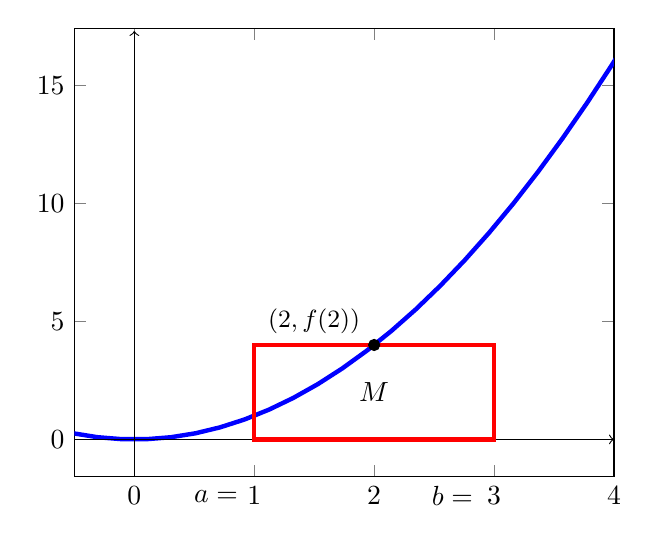
\begin{tikzpicture}
						\begin{axis}[xmin=-1/2, xmax=4, samples=50]
						  	\addplot[blue, ultra thick] (x, x*x);
						  	\draw[->] (-2, 0) -- (4, 0);
						  	\draw[->] (0, -2) -- (0, 17.3);
						  	
						  	\draw[red, ultra thick] (1, 0) rectangle (3, 4);
						  	
					  		\draw (2, 4) circle[radius=2pt];
					  		\fill (2, 4) circle[radius=2pt];
					  		\node at (2, 2) {$M$};
					  		\node at (1.5, 5) {\small $(2, f(2))$};
						\end{axis}
						
						\node at (1.8, -1/4) {\normalsize $a=$};
						\node at (4.8, -1/4) {\normalsize $b=$};
					\end{tikzpicture}
				\end{figure}
			\end{column}
			
			\begin{column}{0.5\textwidth}
				\begin{align*}
					M &= \overbrace{(b-a) \cdot f\left(\frac{b+a}{2}\right)}^{\text{area of a rectangle!}} \\
					&= \Delta x \cdot f(m)	
				\end{align*}

			\end{column}
		\end{columns}

	\end{frame}
	
	\begin{frame}[c]{Trapezoid rule} \centering
		\begin{columns}[c]
			\begin{column}{0.5\textwidth}
				\begin{figure}[l]
					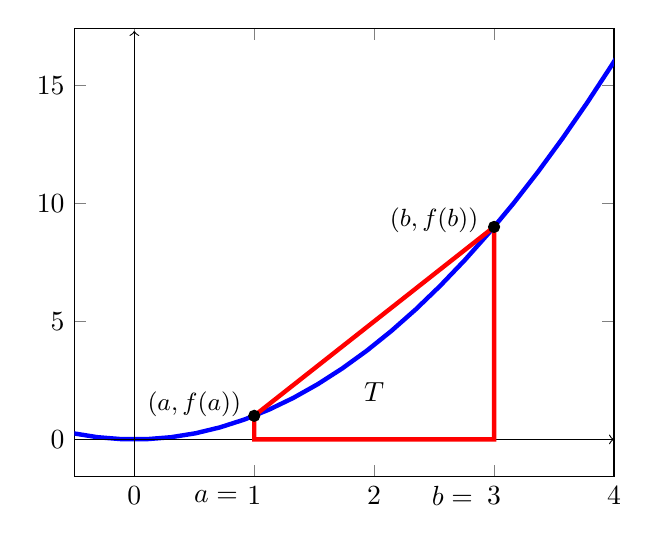
\begin{tikzpicture}
						\begin{axis}[xmin=-1/2, xmax=4, samples=50]
						  	\addplot[blue, ultra thick] (x, x*x);
						  	\draw[->] (-2, 0) -- (4, 0);
						  	\draw[->] (0, -2) -- (0, 17.3);
						  	
						  	\node (a) at (1, 0) {};
						  	\node (b) at (1, 1) {};
						  	\node (c) at (3, 9) {};
						  	\node (d) at (3, 0) {};
						  	\draw[red, ultra thick] (a.center) -- (b.center) -- (c.center) -- (d.center) -- cycle;
						  	
					  		\node at (2, 2) {$T$};
					  		
					  		\node at (0.5, 1.5) {\small $(a, f(a))$};
					  		\draw (1, 1) circle[radius=2pt];
					  		\fill (1, 1) circle[radius=2pt];
					  		
					  		\node at (2.5, 9.3) {\small $(b, f(b))$};
					  		\draw (3, 9) circle[radius=2pt];
					  		\fill (3, 9) circle[radius=2pt];
						\end{axis}
						
						\node at (1.8, -1/4) {\normalsize $a=$};
						\node at (4.8, -1/4) {\normalsize $b=$};
					\end{tikzpicture}
				\end{figure}
			\end{column}
			
			\begin{column}{0.5\textwidth}
				\begin{align*}
					T &= \overbrace{(b-a) \cdot \frac{f(b) + f(a)}{2}}^{\text{area of a trapezoid!}} \\
					&= \frac{\Delta x}{2} \cdot (f(b) + f(a))
				\end{align*}

			\end{column}
		\end{columns}
	\end{frame}
	
	\begin{frame}[c]{Simpson's rule} \centering
		\begin{columns}[c]
			\begin{column}{0.5\textwidth}
				\begin{figure}[l]
					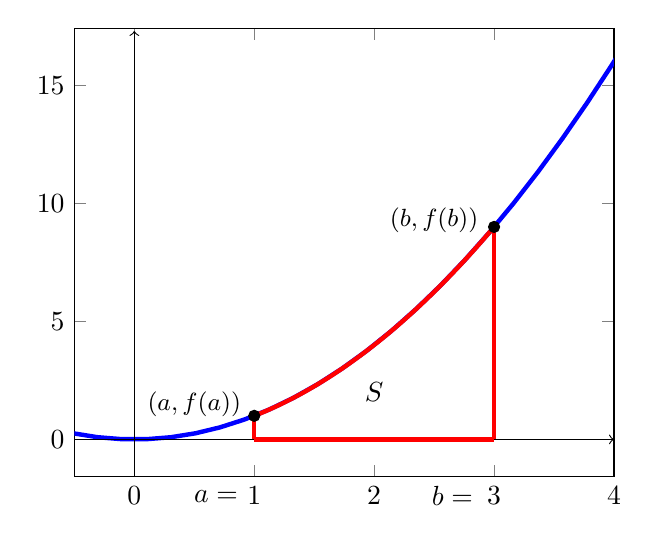
\begin{tikzpicture}
						\begin{axis}[xmin=-1/2, xmax=4, samples=50]
						  	\addplot[blue, ultra thick] (x, x*x);
						  	\draw[->] (-2, 0) -- (4, 0);
						  	\draw[->] (0, -2) -- (0, 17.3);
						  	
						  	\node (a) at (1, 0) {};
						  	\node (b) at (1, 1) {};
						  	\node (c) at (3, 9) {};
						  	\node (d) at (3, 0) {};
						  	\draw[red, ultra thick] (a.center) -- (b.center);
						  	\draw[red, ultra thick] (a.center) -- (d.center);
						  	\draw[red, ultra thick] (c.center) -- (d.center);
						  	
						  	\addplot[red, ultra thick, domain=1:3] (x, x*x);						  	
					  		\node at (2, 2) {$S$};
					  		
					  		\node at (0.5, 1.5) {\small $(a, f(a))$};
					  		\draw (1, 1) circle[radius=2pt];
					  		\fill (1, 1) circle[radius=2pt];
					  		
					  		\node at (2.5, 9.3) {\small $(b, f(b))$};
					  		\draw (3, 9) circle[radius=2pt];
					  		\fill (3, 9) circle[radius=2pt];
						\end{axis}
						
						\node at (1.8, -1/4) {\normalsize $a=$};
						\node at (4.8, -1/4) {\normalsize $b=$};
					\end{tikzpicture}
				\end{figure}
			\end{column}
			
			\begin{column}{0.5\textwidth}
				\begin{align*}
					S &= \overbrace{\frac{b-a}{3} \cdot \frac{f(a) + 4f\left( \frac{b+a}{2} \right) + f(b)}{2}}^{\text{magic!}} \\
					&= \frac{2M + T}{3}
				\end{align*}
			\end{column}
		\end{columns}
	\end{frame}
	
	\begin{frame}[c]{6, old exam 2} \centering \Large
		If $a=0$ and $b=3$, use each rule to estimate the value of $$ \int_0^3 \frac{x}{1+x+x^2} \ dx$$	
	\end{frame}
	
	\begin{frame}[c] \centering \Large
		$$M = \onslide<2->{3 \cdot \frac{\nicefrac 32}{1 + \nicefrac 32 + (\nicefrac 32)^2}}$$
	\end{frame}
	
	\begin{frame}[c] \centering \Large
		$$T = \onslide<2->{3 \cdot \frac{0 + \frac{3}{1+3+9}}{2}}$$
	\end{frame}
	
	\begin{frame}[c]\centering \Large \bf
		8.8 --- improper integrals	
	\end{frame}
	
	\begin{frame}[c] \centering \Large
		$$ \int_a^\infty f(x) \ dx = \lim_{b \to \infty}\left( \int_a^b f(x) \ dx \right) $$	
	\end{frame}
	
	\begin{frame}[c]{7(b), old exam 2} \centering \Large
		use the definition of the improper integral to find the value of $$ \int_0^\infty e^{-st} \ dt $$ when $s > 0$ is a constant.
	\end{frame}

	\begin{frame}
		\begin{align*}
			\int_0^\infty e^{-st} \ dt &= \lim_{b \to \infty} \int_0^b e^{-st} \ dt \\
			aq	qQ\onslide<2->{&=\lim_{b \to \infty} \frac{-1}{s}e^{-st} \Big|^b_0 \\}
			\onslide<3->{&=\lim_{b \to \infty} \left(\frac{-1}{s}e^{-sb} - \frac{-1}{s}e^{-s0} \right) \\}
			\onslide<4->{&=\frac{-1}{s} \cdot 0 + \frac{1}{s}\\}
			 \onslide<5->{&=\frac 1s}
		\end{align*}
	
	\end{frame}



\end{document}
